\documentclass[10pt]{article}
\usepackage{tmlr}

\usepackage{amsmath}
\usepackage{hyperref}
\usepackage{url}
\usepackage{booktabs}
\usepackage{graphicx}

\title{Weaker Language Models Need Colder Sampling}

\author{\name Anonymous authors \email anonymous@anonymous.org}

\def\month{MM}
\def\year{YYYY}
\def\openreview{\url{https://openreview.net/forum?id=XXXX}}

\begin{document}

\maketitle

\begin{abstract}
Language models are usually sampled at a temperature of 0.7 or 1.0, whatever the model. We ask whether the best temperature depends on the model, and if so, whether model size or model quality decides it. For 14 base models from 70M to 2.8B parameters, we find the temperature $T^*$ at which a model's text is exactly as surprising to a stronger judge model as real human text. $T^*$ is below 1 for every model and ranges from 0.62 for the weakest to 0.83 for the best. It follows the model's loss, not its size: two models with the same loss and a 3.5$\times$ difference in parameters have the same $T^*$, and a formula fitted on one model family predicts another to within 0.014. Every experiment ran on one 16GB laptop.
\end{abstract}

\section{Introduction}

We finetuned a 297M-parameter model to chat and asked it the capital of Australia. At temperature 0.7 it said Melbourne, and on another try, Perth. At 0.7 it gave a sensible reply to ``hi'' 8 times out of 12. At 0.4 it did it 12 times out of 12.

Temperature controls how adventurous a model is when it picks the next word. Low temperatures make it stick to likely words. High temperatures let it pick unlikely ones. Most people leave it at 0.7 or 1.0 for every model, but those defaults come from large models. Our small model clearly wanted something colder.

This paper asks: \textbf{does the best sampling temperature depend on how good a language model is, and is it model quality (loss) or model size that decides it?}

We find that:
\begin{itemize}
    \item every model we tested wants a temperature below 1, between 0.62 and 0.83;
    \item better models want hotter temperatures;
    \item what decides it is the model's loss, not its number of parameters;
    \item a simple formula fitted on one family of models predicts the best temperature for another.
\end{itemize}

\section{Related work}

Sampling straight from a language model's probabilities tends to produce strange text, because the model gives a little probability to many bad words and sometimes picks one~\citep{holtzman2020curious}. The usual fixes lower the temperature or cut off unlikely words, as in top-$k$~\citep{fan2018hierarchical}, nucleus~\citep{holtzman2020curious} and min-$p$~\citep{nguyen2024minp} sampling. Mirostat~\citep{basu2021mirostat} adjusts sampling as it goes to keep the text at a target level of surprise, which is the closest idea to ours, but the target has to be picked by hand. \citet{li2025hot} found that bigger models keep their benchmark scores at higher temperatures, which fits what we see.

The work closest to ours is \citet{cao2025entropy}, building on \citet{braverman2020calibration}. They measure whether a model is consistent with itself: whether it is as surprised by its own writing as by real text. They find that the temperature that fixes this is about the same for every model size. We measure something different: whether a model's writing matches human writing, judged by a stronger model. A model can be consistent with itself and still be wrong about the world, so the two answers do not have to agree. In our results, they don't.

\section{Method}

\paragraph{Text.} We took 200 passages from WikiText-103~\citep{merity2016pointer}, a collection of Wikipedia articles. Each passage gives a 40-word prompt and the 80 words that really came next.

\paragraph{Models.} Six Pythia models from 70M to 2.8B parameters~\citep{biderman2023pythia}, Pythia-410M saved at training steps 4k, 16k and 64k, Pythia-1.4B at step 16k, three SmolLM2 models (135M, 360M and 1.7B)~\citep{allal2025smollm2}, and a 297M model we pretrained ourselves. That is 14 models in total.

\paragraph{Generating.} Each model continued every prompt at 15 temperatures, from 0.1 to 1.5 in steps of 0.1, with no other sampling tricks. We kept the first 80 words of each continuation.

\paragraph{Judging.} A larger model, Qwen2.5-3B~\citep{qwen2025qwen25}, read every continuation and measured how surprising it was, in bits per byte. Bits per byte lets us compare models with different tokenizers. The judge also read the real human continuations, which scored 0.766 bits per byte.

\paragraph{Finding $T^*$.} As temperature rises, a model's writing gets more surprising to the judge. $T^*$ is the temperature where it becomes exactly as surprising as the human text (Figure~\ref{fig:curves}). We resampled the prompts 300 times to get a 95\% range for each $T^*$.

\paragraph{Model quality.} A model's loss is how surprised the model itself is by the real human continuations, also in bits per byte. Lower loss means a better model.

\paragraph{Hardware.} Everything ran overnight on one MacBook Air with 16GB of memory.

\begin{figure}[t]
\centering
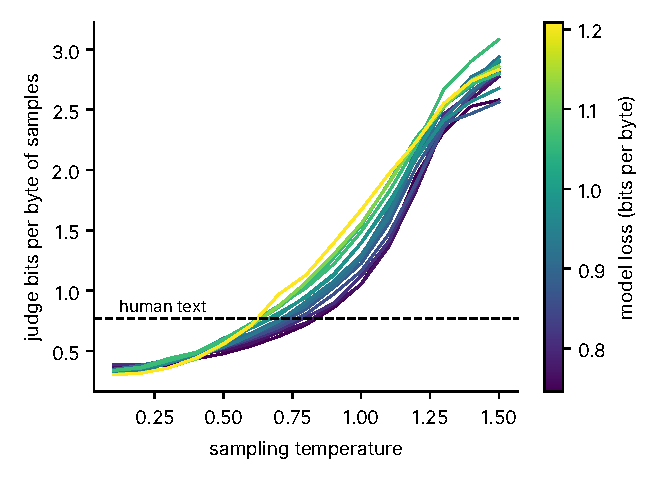
\includegraphics[width=0.55\linewidth]{figs/curves.pdf}
\caption{How surprising each model's writing is to the judge as temperature rises. Colour shows the model's loss. The dashed line is real human text. Each model's $T^*$ is where its curve crosses the line. Worse models cross earlier.}
\label{fig:curves}
\end{figure}

\section{Results}

\subsection{Every model wants a temperature below 1}

At temperature 1.0, every model's writing was far more surprising than human text: from 1.05 bits per byte for the best models to 1.67 for the worst, against 0.77 for human text. Every model's curve crossed the human line between 0.6 and 0.85 (Figure~\ref{fig:curves}). At the usual default of 0.7, the six weakest models were too hot and the five best were too cold.

\subsection{Better models want hotter temperatures}

Table~\ref{tab:models} lists every model. $T^*$ goes from 0.62 for Pythia-70M, the weakest model, to 0.83 for SmolLM2-1.7B, the best. Figure~\ref{fig:main} shows the pattern.

\begin{table}[t]
\centering
\small
\begin{tabular}{lrrrc}
\toprule
model & parameters & loss & $T^*$ & 95\% range \\
\midrule
SmolLM2-1.7B & 1711M & 0.746 & 0.827 & 0.807--0.842 \\
Pythia-2.8B & 2775M & 0.766 & 0.815 & 0.792--0.833 \\
Pythia-1.4B & 1415M & 0.810 & 0.778 & 0.750--0.806 \\
Pythia-1B & 1012M & 0.856 & 0.764 & 0.746--0.783 \\
SmolLM2-360M & 362M & 0.878 & 0.736 & 0.721--0.751 \\
Pythia-410M & 405M & 0.911 & 0.708 & 0.688--0.724 \\
Pythia-1.4B, step 16k & 1415M & 0.912 & 0.700 & 0.674--0.723 \\
Pythia-410M, step 64k & 405M & 0.932 & 0.706 & 0.682--0.725 \\
SmolLM2-135M & 135M & 0.970 & 0.673 & 0.656--0.695 \\
Pythia-410M, step 16k & 405M & 0.982 & 0.653 & 0.628--0.677 \\
Pythia-160M & 162M & 1.057 & 0.634 & 0.618--0.648 \\
ours & 297M & 1.062 & 0.626 & 0.607--0.639 \\
Pythia-410M, step 4k & 405M & 1.121 & 0.635 & 0.619--0.650 \\
Pythia-70M & 70M & 1.208 & 0.622 & 0.608--0.632 \\
\bottomrule
\end{tabular}
\caption{All 14 models, from best to worst. Loss is in bits per byte on the human text (lower is better). $T^*$ is the best temperature.}
\label{tab:models}
\end{table}

\begin{figure}[t]
\centering
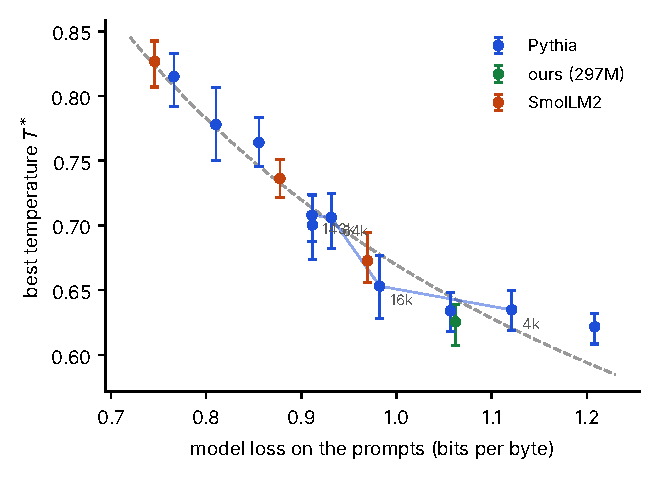
\includegraphics[width=0.62\linewidth]{figs/tstar_loss.pdf}
\caption{Best temperature against model loss. Error bars show the 95\% range. The thin line joins four saved versions of Pythia-410M from the same training run, labelled by training step. The dashed curve is the formula in Section~\ref{sec:formula}.}
\label{fig:main}
\end{figure}

\subsection{Loss decides it, not size}

Pythia-1.4B at training step 16k and the finished Pythia-410M have almost exactly the same loss (0.912 and 0.911), but one is 3.5 times bigger than the other. Their best temperatures are also the same: 0.700 and 0.708. A second pair shows the same thing: SmolLM2-135M and Pythia-410M at step 16k have similar loss (0.970 and 0.982), are 3 times apart in size, and want similar temperatures (0.673 and 0.653).

Across all 14 models, loss predicts $T^*$ well ($r^2 = 0.95$). Size on its own does much worse ($r^2 = 0.68$), and once you know the loss, knowing the size adds almost nothing (Figure~\ref{fig:size}).

\begin{figure}[t]
\centering
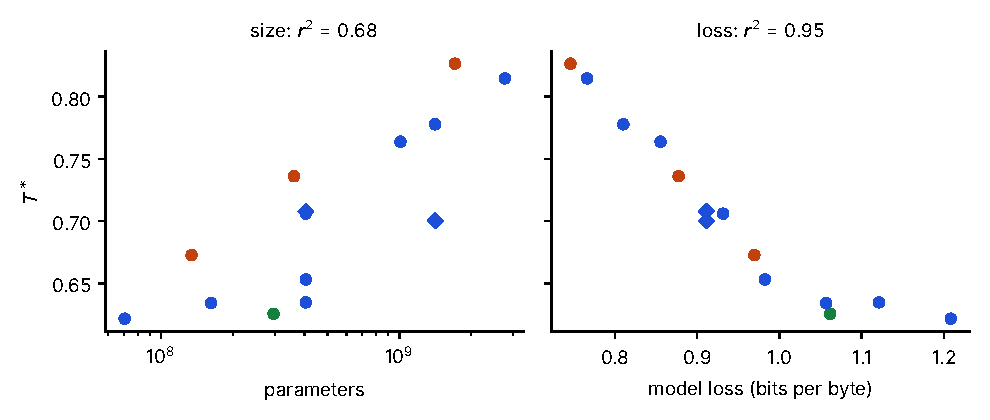
\includegraphics[width=0.85\linewidth]{figs/size_vs_loss.pdf}
\caption{Best temperature against size (left) and against loss (right). The diamonds are two models with the same loss and a 3.5$\times$ difference in size.}
\label{fig:size}
\end{figure}

\subsection{One model, getting better}

The clearest test keeps the model the same and only changes how long it has been trained. Pythia-410M at steps 4k, 16k, 64k and 143k (finished) has loss 1.121, 0.982, 0.932 and 0.911, and its best temperature goes 0.635, 0.653, 0.706 and 0.708. As the same model learns, it wants a hotter temperature, and it follows the same line as all the other models (Figure~\ref{fig:main}).

\subsection{A formula}
\label{sec:formula}

A simple formula fits all 14 models:
\[
T^* \approx 0.22 + 0.59 \times \frac{\text{judge's loss on human text}}{\text{model's loss}}.
\]
To check it isn't just fitting noise, we fitted it on the 10 Pythia models only and used it to predict the others. It predicted the three SmolLM2 models to within 0.014, all inside their 95\% ranges. Our own model came out 0.022 colder than predicted, just outside its range.

\section{Discussion}

\paragraph{Why do weaker models need colder temperatures?} A model trained on text learns to put some probability on many words, so that it is never completely surprised. A weaker model has to spread its bets wider. When you sample from it, those wide bets sometimes land on words a human would never write. Lowering the temperature pulls the model back toward its most confident words. The worse the model, the more it needs pulling back.

\paragraph{Why do \citet{cao2025entropy} find the same temperature for every size?} They ask whether a model's writing matches what the model itself expects. A model trained this way always roughly agrees with itself, however good or bad it is, a bit like a student marking their own homework with their own answer key. Our judge is an outside reader that knows real text better than the models do, so it notices how wrong a weak model's writing is.

\paragraph{What to do with this.} If you run a small model, sample it colder than 0.7. If you know your model's loss and have a stronger model to compare against, the formula gives a starting point.

\section{Limitations}

\begin{itemize}
    \item \textbf{The judge is not much stronger than the best models.} SmolLM2-1.7B beat Qwen2.5-3B on this text, and Pythia-2.8B tied it, so the results for the best models are the least reliable.
    \item \textbf{The text is old.} WikiText is old Wikipedia, which some of these models probably saw in training. That could make their loss look better than it really is.
    \item \textbf{``Best'' is defined by the judge.} We have not yet tested whether people actually prefer text written at $T^*$.
    \item \textbf{Small scope.} One kind of text, base models only (no chat models), at most 2.8B parameters, short continuations, and the four largest models only got 100 prompts each.
\end{itemize}

We plan to repeat the experiment on Wikipedia articles written in 2026, which no model could have seen, with a stronger judge, and to test whether people prefer text at $T^*$.

\section{Conclusion}

There is no single right temperature. Every model we tested wanted less than 1, and better models wanted more than worse ones. What decides it is how good the model is, not how big it is. For small models, that means sampling colder than most people do.

\bibliography{refs}
\bibliographystyle{tmlr}

\end{document}
